\chapter{Farben und Zufallszahlen}
\renewcommand{\chaptertitle}{Farben und Zufallszahlen}

\lehead[]{\sf\hspace*{-2.00cm}\textcolor{white}{\colorbox{lightblue}{\makebox[1.60cm][r]{\thechapter}}}\hspace{0.17cm}\textcolor{lightblue}{\chaptertitle}}
\rohead[]{\textcolor{lightblue}{\chaptertitle}\sf\hspace*{0.17cm}\textcolor{white}{\colorbox{lightblue}{\makebox[1.60cm][l]{\thechapter}}}\hspace{-2.00cm}}
%\chead[]{}
\rehead[]{\textcolor{lightblue}{AvHG, Inf, My}}
\lohead[]{\textcolor{lightblue}{AvHG, Inf, My}}

\lstset{style=myJava}

\section{Farben}

\subsection{Standardfarben}

Farben werden in Java mit der Klasse \myClass{Color} gemischt. In der Klasse
gibt es bereits vordefinierte Konstanten für die Standardfarben, die man z.B.
in eine Variable hinein schreiben kann. Beispiel:

\begin{lstlisting}
Color rot = Color.RED;   æ// Schreibt die Farbe Rot in die Variable "rot"
\end{lstlisting}

Die Variable \lstinline|rot| kann man dann z.B. innerhalb der
\lstinline|myPaint()|-Methode zum Wechseln der Farbe verwenden:

\begin{lstlisting}
g.setColor(rot);
\end{lstlisting}


\subsection{Farben Mischen}

Wenn man eine Farbe mischen möchte, so muss man ein neues \myClass{Color}-Objekt
erzeugen und dabei als Parameter die RGB-Werte (rot, grün, blau) angeben. 

\begin{center}
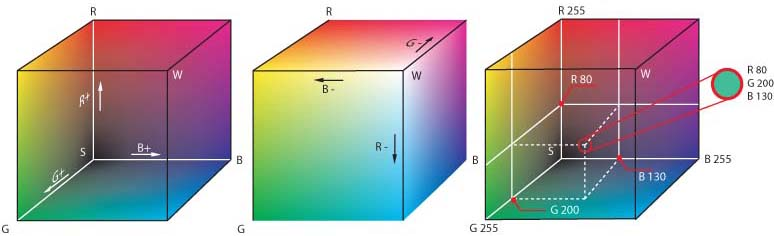
\includegraphics[width=0.9\textwidth]{./inf/SEKII/09_Java_Farben_und_Zufall/RGB_farbwuerfel.jpg}
% http://commons.wikimedia.org/wiki/File:RGB_farbwuerfel.jpg
\end{center}

Beispiel:

\begin{lstlisting}
Color hellrot = new Color(255,180,180);
\end{lstlisting}

Die Variable \lstinline|hellrot| kann man dann z.B. innerhalb der
\lstinline|myPaint()|-Methode zum Wechseln der Farbe verwenden:

\begin{lstlisting}
g.setColor(hellrot);
\end{lstlisting}


\section{Zufallszahlen}

\begin{compactenum}[a)]
\item Um Zufallszahlen zu verwendet, benötigt man oben in der Datei die folgende
 Import-Anweisung:

\begin{lstlisting}
import java.util.Random;
\end{lstlisting}

\item Bei den globalen Variablen muss man eine Variable der Klasse
\myClass{Random} anlegen und für diese Variable ein Objekt erzeugen. Dies ist
quasi der „Zufallsgenerator“ mit dem man sich später die Zufallszahlen
generieren kann.

\begin{lstlisting}
Random zufallsgenerator = new Random();
\end{lstlisting}

\item Ganzzahlige Zufallszahlen erhält man, wenn man auf das
Zufallsgenerator-Objekt die folgende Methode anwendet:

\begin{lstlisting}
public int nextInt(int n)   æ// Erzeugt eine Zufallszahl von 0 bis n-1
\end{lstlisting}

Beispiele:

\begin{lstlisting}
int zufallA = zufallsgenerator.nextInt(5);    æ// Zufallszahl zwischen 0 und 4
æint zufallB = zufallsgenerator.nextInt(5)+2;  æ// Zufallszahl zwischen 2 und 6
\end{lstlisting}
\end{compactenum}
